\documentclass[a4paper,12pt]{article}
\usepackage{docsTemplate}
\usepackage{longtable}
\usepackage{float}
\usepackage[official]{eurosym}
\usepackage{pgf-pie}
\usepackage{makecell}

\usepackage{titlesec}

\titleformat{\paragraph}[block]
  {\normalfont\normalsize\bfseries}
  {\theparagraph}{1em}{}

\titlespacing*{\paragraph}{0pt}{3.25ex plus 1ex minus .2ex}{1.5ex}

\setTitle{Piano di Progetto}
\setAuthors{Bianca Zaghetto}
\setVerificators{Mattia Oliva
Medin \\ & Sara Gioia
Fichera \\ & Andrea Masiero}
\setApprovation{}
\setVersion{0.6}
\setType{Esterno}
\setDestination{Tullio Vardanega \\ & Riccardo Cardin \\ & Sanmarco Informatica \\[-0.1em] & Team Three Technologies}
\setcounter{secnumdepth}{4}
\setcounter{tocdepth}{4}

\begin{document}
\include{docTitlepage}

\newpage
\section*{Registro delle modifiche}

\begin{table}[h!]
\rowcolors{2}{lightgray}{white}
\begin{tabularx}{\textwidth}{|l|l|l|l|L|L|}
\hline
\textbf{Vers.} & \textbf{Data} & \textbf{Autore} & \textbf{Ruolo} & \textbf{Verifica} & \textbf{Oggetto} \\
\hline
\textbf{0.6} & 21/12/25 & Bianca Zaghetto & Verificatore & Andrea Masiero & Aggiunta pianificazione secondo periodo \\
\hline
\textbf{0.5} & 20/12/25 & Bianca Zaghetto & Verificatore & Andrea Masiero & Aggiunta pianificazione primo periodo \\
\hline
\textbf{0.4} & 15/12/25 & Bianca Zaghetto & Verificatore & Andrea Masiero & Sezione orario previsto e stima costi \\
\hline
\textbf{0.3} & 09/12/25 & Bianca Zaghetto & Verificatore & Sara Gioia Fichera & Sezione calendario \\
\hline
\textbf{0.2} & 02/12/25 & Bianca Zaghetto & Verificatore & Sara Gioia Fichera & Sezione introduttiva e sezione rischi attesi \\
\hline
\textbf{0.1} & 27/11/25 & Bianca Zaghetto & Verificatore & Mattia Oliva Medin & Prima stesura: struttura documento \\
\hline
\end{tabularx}
\end{table}

\newpage
\tableofcontents

\newpage
\listoffigures

\newpage
\listoftables

\newpage

\section{Introduzione}
    \subsection{Scopo del documento}
        Il presente documento ha lo scopo di tenere traccia e definire le modalità di svolgimento delle attività nonché la suddivisione delle risorse in esse impiegate.
        Per la stesura del Piano di Progetto viene applicato un approccio incrementale, integrando informazioni fino al termine del progetto. Il documento tratta i seguenti temi:
        \begin{itemize}
            \item Rischi attesi e loro mitigazione
            \item Calendario di massima del progetto
            \item Impegno orario previsto e stima dei costi totali
            \item Periodi di avanzamento
            \item Consuntivo di periodo
            \item Preventivo
        \end{itemize}
    \subsection{Glossario}
        Per definizioni esaustive dei termini utilizzati in questo documento, si rimanda al Glossario disponibile nella documentazione. Tutti i termini che si possono trovare in esso vengono identificati da una G a pedice.
    \subsection{Riferimenti}
        \subsubsection{Riferimenti normativi}
            \begin{itemize}
                \item \href{https://team-three-technologies.github.io/Documenti/1%20-%20RTB/Norme_di_progetto_v0_4.pdf}{Norme di Progetto} (Ultimo accesso: 11/01/2026)
                \item \href{https://www.math.unipd.it/~tullio/IS-1/2025/Dispense/PD1.pdf}{Regolamento del progetto didattico} (Ultimo accesso: 11/01/2026)
            \end{itemize}
        \subsubsection{Riferimenti informativi}
            \begin{itemize}
                \item \href{https://team-three-technologies.github.io/Documenti/1%20-%20RTB/Analisi_dei_Requisiti_v0_1.pdf}{Analisi dei Requisiti} (Ultimo accesso: 08/01/2026)
                \item Verbali interni
                \item Verbali esterni
                \item \href{https://www.math.unipd.it/~tullio/IS-1/2025/Progetto/C3.pdf}{Capitolato C3} (Ultimo accesso: 10/01/2026)
                \item \href{https://www.math.unipd.it/~tullio/IS-1/2025/Dispense/T02.pdf}{Processi di ciclo di vita del \textit{software}} (Ultimo accesso: 05/01/2026)
                \item \href{https://www.math.unipd.it/~tullio/IS-1/2025/Dispense/T04.pdf}{Gestione di progetto} (Ultimo accesso: 07/01/2026)
            \end{itemize}

\newpage
\section{Rischi attesi e loro mitigazione}
\label{sec:rischi}
    \subsection{Introduzione}
        In questa sezione vengono elencati i rischi che si potrebbero incontrare durante lo svolgimento del progetto, corredati dalla possibile mitigazione relativa.
        
        Per rendere facilmente fruibile il documento, viene associato un codice identificativo univoco ad ogni rischio.
    \subsection{R1 - Tecnologie di lavoro e di produzione SW}
        \begin{table}[H]
        \rowcolors{2}{lightgray}{white}
        \label{tab:r1} 
            \begin{tabularx}{\textwidth}{|l|L|L|L|}
            \hline
            \textbf{Codice} & \textbf{Oggetto} & \textbf{Descrizione} & \textbf{Mitigazione}\\
            \hline
            \textbf{R1-1} & Inesperienza nelle tecnologie da utilizzare & Uno o più membri del gruppo si trovano in difficoltà nell'utilizzo delle tecnologie scelte & Studio personale e condivisione delle conoscenze\\
            \hline
            \textbf{R1-2} & Problemi tecnici software o hardware & Uno o più membri del gruppo riscontrano problemi tecnici con strumenti software o hardware & Si provvederà ad aggiornare il gruppo sul problema riscontrato. Qualora il membro o i membri siano impossibilitati a portare a termine un obiettivo, dovranno trovare una soluzione alternativa o cedere l'incarico a qualcun altro finché non avranno risolto il problema.\\            
            \hline
            \end{tabularx}
            \caption{Rischi sulle tecnologie di lavoro e di produzione SW}
        \end{table}
        
    \subsection{R2 - Rapporti interpersonali}
        \begin{table}[H]
        \rowcolors{2}{lightgray}{white}
        \label{tab:r2}
            \begin{tabularx}{\textwidth}{|l|L|L|L|}
            \hline
            \textbf{Codice} & \textbf{Oggetto} & \textbf{Descrizione} & \textbf{Mitigazione}\\
            \hline
            \textbf{R2-1} & Divergenze di pensiero & Il gruppo non riesce a giungere ad una decisione unanime per divergenze di pensiero & Utilizzo di sondaggi gestiti dal responsabile o, in casi estremi, richiesta di intervento da parte del docente/proponente\\
            \hline
            \textbf{R2-2} & Mancanza di riscontro & Uno o più membri del gruppo non danno riscontro rispetto agli incarichi assegnati & Promemoria regolari, se necessario per canali privati o in presenza. In casi estremi verrà contattato il docente.\\
            \hline
            \textbf{R2-3} & Abbandono del progetto & Uno o più membri del gruppo decidono di abbandonare il progetto per motivi personali & Verrà contattato il docente per rendere nota la situazione e si provvederà, se necessario, a valutare insieme alla proponente una negoziazione dei requisiti richiesti \\
            \hline
            \end{tabularx}
            \caption{Rischi sui rapporti interpersonali}
        \end{table}
        
    \subsection{R3 - Organizzazione del lavoro}
        \begin{table}[H]
        \rowcolors{2}{lightgray}{white}
        \label{tab:r3}
            \begin{tabularx}{\textwidth}{|l|L|L|L|}
            \hline
            \textbf{Codice} & \textbf{Oggetto} & \textbf{Descrizione} & \textbf{Mitigazione}\\
            \hline
            \textbf{R3-1} & Assenze alle riunioni esterne/interne & Uno o più membri del gruppo non presenziano alle riunioni interne/esterne & Condivisione appunti e registrazioni delle riunioni per permettere il recupero di quanto svolto\\
            \hline
            \textbf{R3-2} & Isolamento & Un membro si isola dal gruppo, non risponde alle comunicazioni, non presenzia costantemente alle riunioni e non svolge gli incarichi previsti & Confronto diretto sulle cause dell'isolamento, analisi delle possibili soluzioni ed eventuale riorganizzazione. In casi gravi, si provvederà a contattare il docente per decidere come procedere\\
            \hline
            \end{tabularx}
            \caption{Rischi sull'organizzazione del lavoro}
        \end{table}
        
    \subsection{R4 - Requisiti e rapporti con gli stakeholder}
        \begin{table}[H]
        \rowcolors{2}{lightgray}{white}
        \label{tab:r4}
            \begin{tabularx}{\textwidth}{|l|L|L|L|}
            \hline
            \textbf{Codice} & \textbf{Oggetto} & \textbf{Descrizione} & \textbf{Mitigazione}\\
            \hline
            \textbf{R4-1} & Malcomprensione requisiti & Il gruppo non comprende appieno i requisiti richiesti o li comprende in modo sbagliato & Utilizzo del form per la comunicazione asincrona con la proponente, ponendo dubbi e domande. Analisi dettagliata dei requisiti con la proponente nel corso delle riunioni. In casi eccezionali, richiesta di riunioni aggiuntive.\\
            \hline
            \end{tabularx}
            \caption{Rischi sui requisiti e rapporti con gli stakeholder}
        \end{table}
        
    \subsection{R5 - Tempi e costi}
        \begin{table}[H]
        \rowcolors{2}{lightgray}{white}
        \label{tab:r5}
            \begin{tabularx}{\textwidth}{|l|L|L|L|}
            \hline
            \textbf{Codice} & \textbf{Oggetto} & \textbf{Descrizione} & \textbf{Mitigazione}\\
            \hline
            \textbf{R5-1} & Ritardo di consegna & Uno o più membri del gruppo non riescono a completare una consegna nei tempi previsti & Qualora possibile, si concederà del tempo aggiuntivo per completare la consegna. Altrimenti si procederà ad affiancare un membro del gruppo disponibile o, in casi estremi, ad effettuare una sostituzione\\
            \hline
            \textbf{R5-2} & Superamento budget & Per il completamento del progetto è richiesto un budget superiore a quello preventivato & Negoziazione al ribasso sui requisiti del progetto con il proponente \\
            \hline
            \end{tabularx}
            \caption{Rischi su tempi e costi}
        \end{table}

    \subsection{Tabella riassuntiva}
        Nella seguente tabella vengono valutati i rischi sopra elencati in base alla loro probabilità di occorrenza e alla loro pericolosità. Entrambe le caratteristiche si suddividono in tre livelli:
        \begin{itemize}
            \item Alto
            \item Medio
            \item Basso
        \end{itemize}

        \begin{table}[H]
        \rowcolors{1}{lightgray}{white}
        \centering
        \label{tab:riass_rischi}
            \begin{tabular}{|l|l|l|}
            \hline
            \textbf{Codice} & \textbf{Livello occorrenza} & \textbf{Livello pericolosità}\\
            \hline
            \textbf{R1-1} & Alto & Medio \\
            \hline
            \textbf{R1-2} & Basso & Medio \\
            \hline
            \textbf{R2-1} & Medio & Basso \\
            \hline
            \textbf{R2-2} & Basso & Medio \\
            \hline
            \textbf{R2-3} & Basso & Alto \\
            \hline
            \textbf{R3-1} & Medio & Basso \\
            \hline
            \textbf{R3-2} & Basso & Alto \\
            \hline
            \textbf{R4-1} & Alto & Medio \\
            \hline
            \textbf{R5-1} & Alto & Alto \\
            \hline
            \textbf{R5-2} & Alto & Medio \\
            \hline
            \end{tabular}
            \caption{Tabella riassuntiva dei rischi}
        \end{table}

\newpage
\section{Calendario di massima del progetto}
    \subsection{Introduzione}
        In questa sezione vengono esposte le date previste per le revisioni del progetto, considerando quanto visto in \href{sec:rischi}{\textit{Rischi attesi e loro mitigazione}} e \href{sec:pianificazione}{\textit{Pianificazione}}.
    \subsection{Stesura iniziale}
        Gli obiettivi iniziali prefissati dal gruppo, per quanto concerne il calendario, sono i seguenti:
        \begin{table}[H]
            \centering
            \label{tab:cal1}
            \begin{tabular}{|c|c|}
            \hline
                \rowcolor{lightgray}{\textbf{Revisione}} & {\textbf{Data}}  \\
            \hline
                Requirements and Technology Baseline & 19/01/2026 \\
            \hline
                Product Baseline & 27/03/2026 \\
            \hline
            \end{tabular}
            \caption{Previsione iniziale delle date di consegna delle revisioni}
        \end{table}

    % \subsection{Prima Revisione}
    %     \begin{table}[H]
    %         \centering
    %         \begin{tabular}{|c|c|}
    %         \hline
    %             \rowcolor{lightgray}{\textbf{Revisione}} & {\textbf{Data}}  \\
    %         \hline
    %             Product Baseline & ???\\
    %         \hline
    %         \end{tabular}
    %         \caption{Data di consegna prevista aggiornata a seguito della RTB}
    %         \label{tab:cal2}
    %     \end{table}

\newpage
\section{Impegno orario previsto e stima dei costi totali}
    \subsection{Introduzione}
        I contenuti di questa sezione si basano su quanto affrontato in \href{sec:rischi}{\textit{Rischi attesi e loro mitigazione}} e nei paragrafi "Preventivo" della sezione \href{sec:prev}{\textit{Pianificazione}}. Gli argomenti cardine sono i seguenti:
        \begin{itemize}
            \item l'impegno orario preventivato, suddiviso per ruoli
            \item la conseguente stima dei costi totali 
        \end{itemize}
    \subsection{Stesura iniziale}
        \begin{table}[H]
        \centering
        \label{tab:costi1}
        \begin{tabular}{|l|c|c|c|}
        \hline
            \rowcolor{lightgray}{\textbf{Ruolo}} & {\textbf{Costo}} & {\textbf{Ore previste}} & {\textbf{Costo totale}} \\
        \hline
            Responsabile & 30\euro{}/h & 64 & 1920\euro{} \\
        \hline
            Amministratore & 20\euro{}/h & 64 & 1280\euro{} \\
        \hline
            Analista & 25\euro{}/h & 80 & 2000\euro{} \\
        \hline
            Progettista & 25\euro{}/h & 124 & 3100\euro{} \\
        \hline
            Programmatore & 15\euro{}/h & 164 & 2460\euro{} \\
        \hline
            Verificatore & 15\euro{}/h & 148 & 2220\euro{} \\
        \hline
            \textbf{Totale} & & 644 & 12980\euro{} \\
        \hline
        \end{tabular}
        \caption{Impegno orario e costi previsti}
        \end{table}

        \begin{figure}[H]
            \centering
            \label{fig:costi1}
            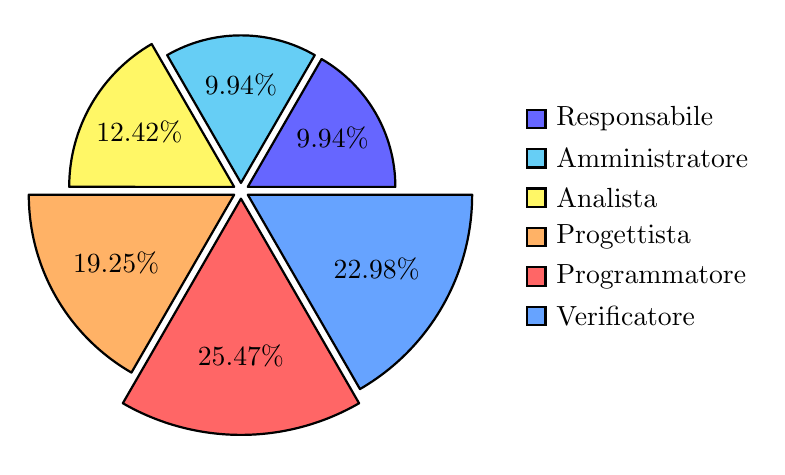
\begin{tikzpicture}
            \pie [polar, explode=0.1, text=legend] { 9.94/Responsabile, 9.94/Amministratore, 12.42/Analista, 19.25/Progettista, 25.47/Programmatore, 22.98/Verificatore }
            \end{tikzpicture}
            \caption{Suddivisione delle ore dei ruoli in percentuale}
        \end{figure}

    La stima per il costo totale del progetto è di 12980\euro{}.

\newpage
\section{Pianificazione}
\label{sec:pianificazione}
    \subsection{Introduzione}
    Questa sezione raccoglie tutte le informazioni relative ad ogni periodo di lavoro svolto dal gruppo, offrendone una rappresentazione chiara e completa.
    \subsection{Requirements and Technology Baseline}

    % PRIMO PERIODO ----------------------------
        \subsubsection{04/11/2025 - 16/11/2025 - Primo periodo}
            \paragraph{Panoramica e obiettivi}
            L'inizio del primo periodo coincide con l'aggiudicazione dell'appalto per il capitolato, a cui è seguita una riunione interna per fissare gli obiettivi di lavoro per le due settimane successive, ovvero:
                \begin{itemize}
                    \item Correzioni alla documentazione
                    \item Inizio stesura Glossario
                    \item Studio delle tecnologie proposte dall'azienda
                \end{itemize}
            Inoltre si è svolta una riunione esterna con la proponente, la quale ha permesso un'organizzazione chiara fin dal principio - modalità di comunicazione sincrona/asincrona e calendarizzazione incontri.
            \paragraph{Gestione rischi}
            \paragraph*{Rischi attesi}
                \begin{itemize}
                    \item\hyperref[tab:r1]{[R1-1] Inesperienza nelle tecnologie da utilizzare}
                    \item\hyperref[tab:r2]{[R2-1] Divergenze di pensiero}
                \end{itemize}
                Per il primo periodo, il gruppo ha previsto un'iniziale inesperienza nelle tecnologie da utilizzare e possibili divergenze di pensiero riguardo le attività da svolgere e la loro suddivisione.

            \paragraph*{Rischi incontrati}
                Si è solamente riscontrata inesperienza nelle tecnologie da utilizzare (R2-1). I membri del gruppo hanno provveduto ad aiutarsi vicendevolmente nel migliorare la dimestichezza con gli strumenti di lavoro.                
            \paragraph{Ruoli assegnati}
            I ruoli assegnati per il primo periodo sono i seguenti:
                \begin{table}[H]
                \centering
                \begin{tabular}{|l|l|}
                \hline
                    \rowcolor{lightgray}{\textbf{Ruolo}} & {\textbf{Membro}} \\
                \hline
                    Responsabile & Bianca Zaghetto \\
                \hline
                    Amministratore & Filippo Compagno \\
                \hline
                    Analista & \makecell[l]{Nenad Radulovic \\ Sara Gioia Fichera \\ Francesco Balestro} \\
                \hline
                    Progettista & - \\
                \hline
                    Programmatore & - \\
                \hline
                    Verificatore & \makecell[l]{Mattia Oliva Medin \\ Andrea Masiero} \\
                \hline
                \end{tabular}
                \caption{Ruoli primo periodo}
                \end{table}
            
            \paragraph{Preventivo}
                \begin{table}[H]
                \centering
                \begin{tabular}{|l|c|c|c|c|c|c|c|}
                \hline
                    \rowcolor{lightgray}{\textbf{Membro}} & {\textbf{RE}} & {\textbf{AM}} & {\textbf{AN}} & {\textbf{PRJ}} & {\textbf{PRG}} & {\textbf{VER}} & {\textbf{TOTALE}}\\
                \hline
                    Balestro & & & 5 & & & & 5\\
                \hline
                    Compagno & & 8 & & & & & 8\\
                \hline
                    Fichera & & & 5 & & & & 5\\
                \hline
                    Masiero & & & & & & 6 & 6\\
                \hline
                    Oliva Medin & & & & & & 6 & 6\\
                \hline
                    Radulovic & & & 5 & & & & 5\\
                \hline
                    Zaghetto & 10 & & & & & & 10\\
                \hline
                    \rowcolor{lightgray}\textit{Totale per ruolo} & 10 & 8 & 15 & 0 & 0 & 12 & 45\\
                \hline
                    \rowcolor{lightgray}\textit{Totale costi} & 300 & 160 & 375 & 0 & 0 & 180 & 1015\\
                \hline
                \end{tabular}
                \caption{Preventivo orario primo periodo}
                \end{table}

                \begin{figure}[H]
                \centering
                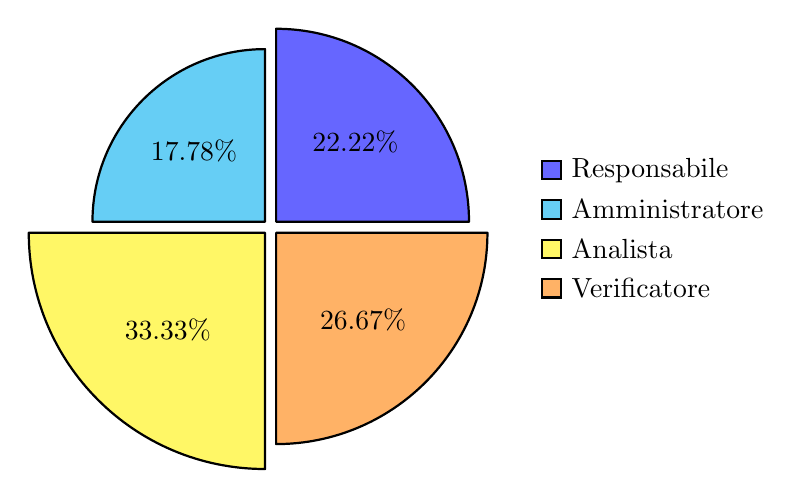
\begin{tikzpicture}
                \pie [polar, explode=0.1, text=legend] { 22.22/Responsabile, 17.78/Amministratore, 33.33/Analista, 26.67/Verificatore }
                \end{tikzpicture}
                \caption{Preventivo orario in percentuale - Primo periodo}
                \end{figure}
        
            \paragraph{Consuntivo}
                \begin{table}[H]
                \centering
                \begin{tabular}{|l|c|c|c|c|c|c|c|}
                \hline
                    \rowcolor{lightgray}{\textbf{Membro}} & {\textbf{RE}} & {\textbf{AM}} & {\textbf{AN}} & {\textbf{PRJ}} & {\textbf{PRG}} & {\textbf{VER}} & {\textbf{TOTALE}}\\
                \hline
                    Balestro & & & 6 & & & & 6\\
                \hline
                    Compagno & & 6 & & & & & 6\\
                \hline
                    Fichera & & & 4 & & & & 4\\
                \hline
                    Masiero & & & & & & 8 & 8\\
                \hline
                    Oliva Medin & & & & & & 5 & 5\\
                \hline
                    Radulovic & & & 4 & & & & 4\\
                \hline
                    Zaghetto & 9 & & & & & & 9\\
                \hline
                    \rowcolor{lightgray}\textit{Totale per ruolo} & 9 & 6 & 14 & 0 & 0 & 13 & 42\\
                \hline
                    \rowcolor{lightgray}\textit{Totale costi} & 270 & 120 & 350 & 0 & 0 & 195 & 935\\
                \hline
                \end{tabular}
                \caption{Consuntivo orario primo periodo}
                \end{table}

                \begin{figure}[H]
                \centering
                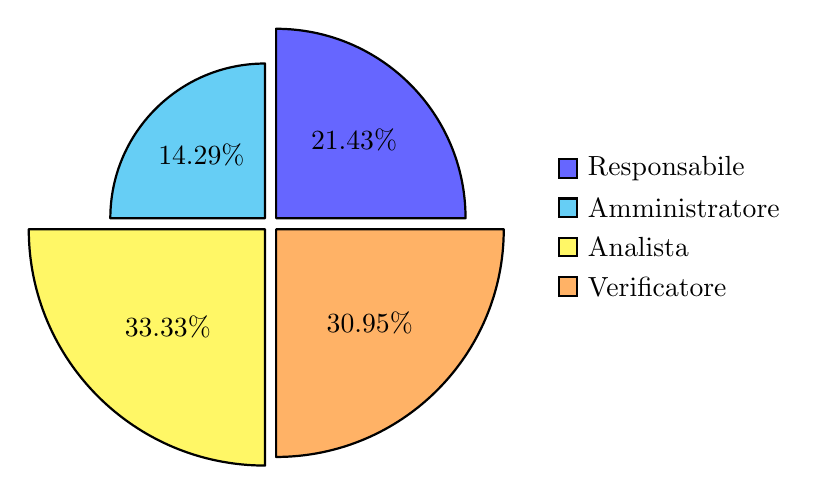
\begin{tikzpicture}
                \pie [polar, explode=0.1, text=legend] { 21.43/Responsabile, 14.29/Amministratore, 33.33/Analista, 30.95/Verificatore }
                \end{tikzpicture}
                \caption{Consuntivo orario in percentuale - Primo periodo}
                \end{figure}
                
            \paragraph{Risorse rimanenti}
                \begin{table}[H]
                \centering
                \begin{tabular}{|l|c|c|}
                \hline
                    \rowcolor{lightgray}{\textbf{Ruolo}} & {\textbf{Ore}} & {\textbf{Costo}}\\
                \hline
                    Responsabile & 9 & 270\\
                \hline
                    Amministratore & 6 & 120\\
                \hline
                    Analista & 14 & 350\\
                \hline
                    Progettista & 0 & 0\\
                \hline
                    Programmatore & 0 & 0\\
                \hline
                    Verificatore & 13 & 195\\
                \hline
                    \rowcolor{lightgray}\textit{Totale} & 42 & 935\\
                \hline
                    \rowcolor{lightgray}\textit{Rimanenti} & 602 & 12045\\
                \hline
                \end{tabular}
                \caption{Risorse economiche rimanenti dal consuntivo orario}
                \end{table}
                
            \paragraph{Retrospettiva}
            Durante il primo periodo il gruppo si è concentrato nello svolgimento degli obiettivi fissati. La documentazione è stata corretta e aggiornata con costanza. Inoltre, si sono svolte riunioni interne per monitorare insieme l'andamento dello studio individuale e delle task assegnate.

    % SECONDO PERIODO --------------------------
        \subsubsection{17/11/2025 - 30/11/2025 - Secondo periodo}
            \paragraph{Panoramica e obiettivi}
            Il secondo periodo è stato caratterizzato dallo studio del materiale fornito dall'azienda e dalla conseguente analisi dei requisiti richiesti. Gli obiettivi fissati sono stati:
                \begin{itemize}
                    \item Aggiornamento delle Norme di Progetto
                    \item Inizio stesura Analisi dei Requisiti
                    \item Inizio stesura Norme di Progetto
                \end{itemize}

            \paragraph{Gestione rischi}
            \paragraph*{Rischi attesi}
                \begin{itemize}
                    \item\hyperref[tab:r4]{[R4-1] Malcomprensione requisiti}
                \end{itemize}
                Per il secondo periodo, il gruppo ha previsto problematiche legate alla stesura dell'Analisi dei Requisiti, dovute ad incomprensioni.

            \paragraph*{Rischi incontrati}
                Come previsto, il gruppo ha trovato difficoltà nell'identificare i casi d'uso previsti (R4-1). Seguendo la mitigazione prevista, ci siamo confrontati con la proponente durante le riunioni in modo da approfondire insieme i requisiti e i casi d'uso.
            
            \paragraph{Ruoli assegnati}
            I ruoli assegnati per il secondo periodo sono i seguenti:
                \begin{table}[H]
                \centering
                \begin{tabular}{|l|l|}
                \hline
                    \rowcolor{lightgray}{\textbf{Ruolo}} & {\textbf{Membro}} \\
                \hline
                    Responsabile & Andrea Masiero \\
                \hline
                    Amministratore & Nenad Radulovic \\
                \hline
                    Analista & \makecell[l]{Mattia Oliva Medin \\ Sara Gioia Fichera \\ Filippo Compagno} \\
                \hline
                    Progettista & - \\
                \hline
                    Programmatore & - \\
                \hline
                    Verificatore & \makecell[l]{Francesco Balestro \\ Bianca Zaghetto} \\
                \hline
                \end{tabular}
                \caption{Ruoli secondo periodo}
                \end{table}
            
            \paragraph{Preventivo}
                \begin{table}[H]
                \centering
                \begin{tabular}{|l|c|c|c|c|c|c|c|}
                \hline
                    \rowcolor{lightgray}{\textbf{Membro}} & {\textbf{RE}} & {\textbf{AM}} & {\textbf{AN}} & {\textbf{PRJ}} & {\textbf{PRG}} & {\textbf{VER}} & {\textbf{TOTALE}}\\
                \hline
                    Balestro & & & & & & 6 & 6\\
                \hline
                    Compagno & & & 5 & & & & 5\\
                \hline
                    Fichera & & & 5 & & & & 5\\
                \hline
                    Masiero & 10 & & & & & & 10\\
                \hline
                    Oliva Medin & & & 5 & & & & 5\\
                \hline
                    Radulovic & & 6 & & & & & 6\\
                \hline
                    Zaghetto & & & & & & 6 & 6\\
                \hline
                    \rowcolor{lightgray}\textit{Totale per ruolo} & 10 & 6 & 15 & 0 & 0 & 12 & 43\\
                \hline
                    \rowcolor{lightgray}\textit{Totale costi} & 300 & 120 & 375 & 0 & 0 & 180 & 975\\
                \hline
                \end{tabular}
                \caption{Preventivo orario secondo periodo}
                \end{table}

                \begin{figure}[H]
                \centering
                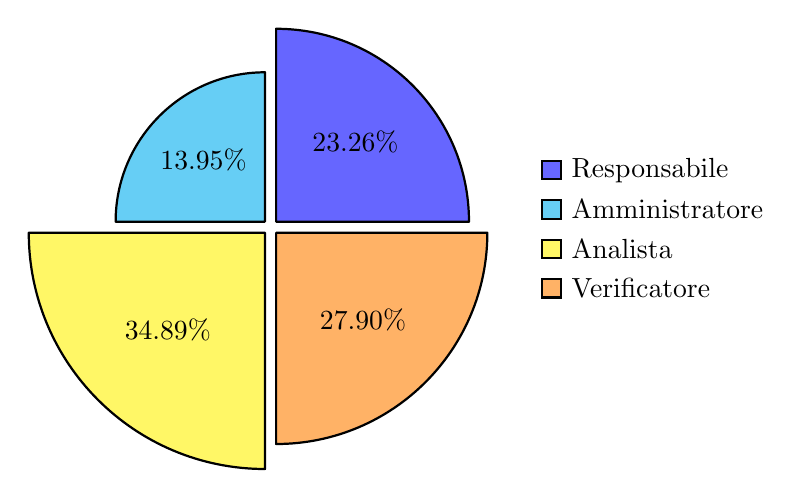
\begin{tikzpicture}
                \pie [polar, explode=0.1, text=legend] { 23.26/Responsabile, 13.95/Amministratore, 34.89/Analista, 27.90/Verificatore }
                \end{tikzpicture}
                \caption{Preventivo orario in percentuale - Secondo periodo}
                \end{figure}
        
            \paragraph{Consuntivo}
                \begin{table}[H]
                \centering
                \begin{tabular}{|l|c|c|c|c|c|c|c|}
                \hline
                    \rowcolor{lightgray}{\textbf{Membro}} & {\textbf{RE}} & {\textbf{AM}} & {\textbf{AN}} & {\textbf{PRJ}} & {\textbf{PRG}} & {\textbf{VER}} & {\textbf{TOTALE}}\\
                \hline
                    Balestro & & & & & & 9 & 9\\
                \hline
                    Compagno & & & 6 & & & & 6\\
                \hline
                    Fichera & & & 4 & & & & 4\\
                \hline
                    Masiero & 9 & & & & & & 9\\
                \hline
                    Oliva Medin & & & 5 & & & & 5\\
                \hline
                    Radulovic & & 8 & & & & & 8\\
                \hline
                    Zaghetto & & & & & & 6 & 6\\
                \hline
                    \rowcolor{lightgray}\textit{Totale per ruolo} & 9 & 8 & 15 & 0 & 0 & 15 & 47\\
                \hline
                    \rowcolor{lightgray}\textit{Totale costi} & 270 & 160 & 375 & 0 & 0 & 225 & 1030\\
                \hline
                \end{tabular}
                \caption{Consuntivo orario secondo periodo}
                \end{table}

                \begin{figure}[H]
                \centering
                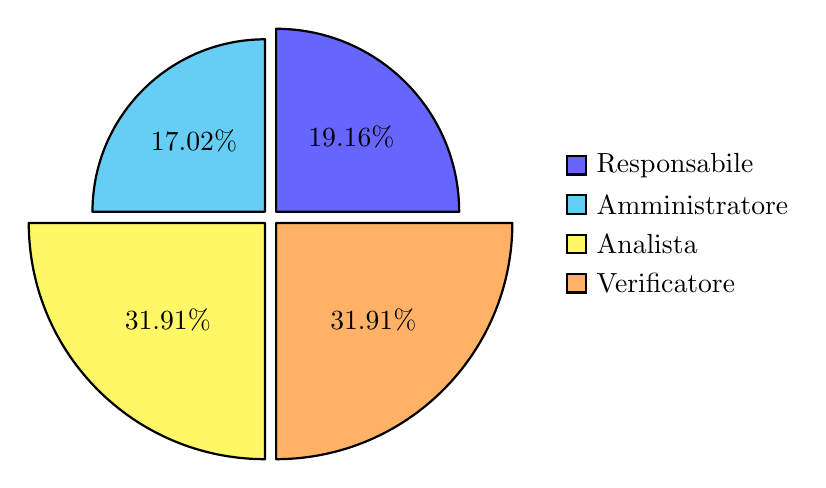
\begin{tikzpicture}
                \pie [polar, explode=0.1, text=legend] { 19.16/Responsabile, 17.02/Amministratore, 31.91/Analista, 31.91/Verificatore }
                \end{tikzpicture}
                \caption{Consuntivo orario in percentuale - Secondo periodo}
                \end{figure}
                
            \paragraph{Risorse rimanenti}
                \begin{table}[H]
                \centering
                \begin{tabular}{|l|c|c|}
                \hline
                    \rowcolor{lightgray}{\textbf{Ruolo}} & {\textbf{Ore}} & {\textbf{Costo}}\\
                \hline
                    Responsabile & 9 & 270\\
                \hline
                    Amministratore & 8 & 160\\
                \hline
                    Analista & 15 & 375\\
                \hline
                    Progettista & 0 & 0\\
                \hline
                    Programmatore & 0 & 0\\
                \hline
                    Verificatore & 15 & 225\\
                \hline
                    \rowcolor{lightgray}\textit{Totale} & 47 & 1030\\
                \hline
                    \rowcolor{lightgray}\textit{Rimanenti} & 555 & 11015\\
                \hline
                \end{tabular}
                \caption{Risorse economiche rimanenti dal consuntivo orario}
                \end{table}
                
            \paragraph{Retrospettiva}
            In questo periodo, la maggiore difficoltà incontrata è stata lo studio e l'interpretazione del materiale fornito dall'azienda, che ha richiesto una buona quantità di studio individuale per essere compreso correttamente. Nonostante ciò, i compiti assegnati sono stati svolti correttamente nei tempi previsti. Il gruppo infatti dimostra spirito di collaborazione e gli incarichi sono stati distribuiti equamente.

    % TERZO PERIODO --------------------------
        \subsubsection{01/12/2025 - 14/12/2025 - Terzo periodo}

    % QUARTO PERIODO --------------------------
        \subsubsection{15/12/2025 - 28/12/2025 - Quarto periodo}

    % QUINTO PERIODO --------------------------
        \subsubsection{29/12/2025 - 11/01/2026 - Quinto periodo}
    
    %\subsection{Product Baseline}
\end{document}
